% !TEX program = pdflatex
% !TEX options = -synctex=1 -interaction=nonstopmode -file-line-error "%DOC%"
% 固体物理第四次作业
\documentclass[UTF8,10pt,a4paper]{article}
\usepackage[scheme=plain]{ctex}
% \catcode`\。=\active
% \newcommand{。}{.}
\newcommand{\CourseName}{固体物理}
\newcommand{\CourseCode}{PHYS1502}
\newcommand{\Semester}{2019-2020学年第二学期}
\newcommand{\ProjectName}{第四次作业}
\newcommand{\DueTimeType}{截止时间}
\newcommand{\DueTime}{2020. 4. 3(周五)17:00}
\newcommand{\StudentName}{陈稼霖}
\newcommand{\StudentID}{45875852}
\usepackage[vmargin=1in,hmargin=.5in]{geometry}
\usepackage{fancyhdr}
\usepackage{lastpage}
\usepackage{calc}
\pagestyle{fancy}
\fancyhf{}
\fancyhead[L]{\CourseName}
\fancyhead[C]{\ProjectName}
\fancyhead[R]{\StudentName}
\fancyfoot[R]{\thepage\ / \pageref{LastPage}}
\setlength\headheight{12pt}
\fancypagestyle{FirstPageStyle}{
    \fancyhf{}
    \fancyhead[L]{\CourseName\\
        \CourseCode\\
        \Semester}
    \fancyhead[C]{{\Huge\bfseries\ProjectName}\\
        \DueTimeType\ : \DueTime}
    \fancyhead[R]{姓名 : \makebox[\widthof{\StudentID}][s]{\StudentName}\\
        学号 : \StudentID\\
        成绩 : \underline{\makebox[\widthof{\StudentID}]{}}}
    \fancyfoot[R]{\thepage\ / \pageref{LastPage}}
    \setlength\headheight{36pt}
}
\usepackage{amsmath,amssymb,amsthm,bm}
\allowdisplaybreaks[4]
\newtheoremstyle{Problem}
{}
{}
{}
{}
{\bfseries}
{.}
{ }
{第\thmnumber{ #2}\thmname{ #1}\thmnote{ (#3)} 得分: \underline{\qquad\qquad}}
\theoremstyle{Problem}
\newtheorem{prob}{题}
\newtheoremstyle{Solution}
{}
{}
{}
{}
{\bfseries}
{:}
{ }
{\thmname{#1}}
\makeatletter
\def\@endtheorem{\qed\endtrivlist\@endpefalse}
\makeatother
\theoremstyle{Solution}
\newtheorem*{sol}{解}
\providecommand{\abs}[1]{\left\lvert#1\right\rvert}
\usepackage{graphicx}
\usepackage{multirow}
\begin{document}
\thispagestyle{FirstPageStyle}
\begin{prob}[(5.2) \textbf{Effective Nuclear Charge and Ionization Energy}]
    \begin{enumerate}
        \item[(a)] Let us approximate an electron in the $n^{th}$ shell (i.e., principal quantum number $n$) of an atom as being like an electron in the $n^{th}$ shell of a hydrogen atom with an effective nuclear charge $Z$. Use your knowledge of the hydrogen atom to calculate the ionization energy of this electron (i.e., the energy required to pull the electron away from the atom) as a function of $Z$ and $n$.
        \item[(b)] Consider the two approximate discussed in the text for estimating the effective nuclear charge:
        \begin{itemize}
            \item (Approximate a)
            \[
                Z=Z_{nuc}-N_{inside}
            \]
            \item (Approximate b)
            \[
                Z=Z_{nuc}-N_{inside}-(N_{same}-1)/2
            \]
            where $Z_{nuc}$ is the actual nuclear charge (or atomic number), $N_{inside}$ is the number of electrons in shells inside of $n$ (i.e., electrons with principal quantum numbers $n'<n$), and $N_{same}$ is the total number of electrons in the $n^{th}$ principal shell (including the electron we are trying to remove from the atom, hence the $-1$).
        \end{itemize}
        \begin{itemize}
            \item[$\triangleright$] Explain the reasoning behind these two approximations.
            \item[$\triangleright$] Use these approximations to calculate the ionization energies for the atoms with atomic number $1$ through $21$. Make a plot of your results and compare them to the actual ionization energies (you will have to look these up on a table).\\
            Your results should be qualitatively quite good. If you try this for higher atomic numbers, the simple approximations begin to break down. Why is this?
        \end{itemize}
    \end{enumerate}
\end{prob}
\begin{sol}
    \begin{enumerate}
        \item[(a)] 将该原子作为氢原子处理,处在第$n$层的电子的电离能为
        \begin{equation}
            E_{\text{ionization}}=\frac{Z^2R}{n^2},
        \end{equation}
        其中$Z$为有效核电荷数,$R=13.6e$V为里德堡常数.
        \item[(b)]
        \begin{itemize}
            \item[$\triangleright$] 在近似情况(a)中,用总电荷减去内层电子数来作为有效核电荷数,这是因为内层原子的轨道有效半径远小于最外层电子的轨道有效半径,因此对于最外层电子来说,原子核与内层电子可以视为一个净电荷数为$Z_{nuc}-N_{inside}$的整体.\\
            在近似情况(b)中,在(a)的基础上进一步减去同层电子数来作为有效核电荷数的一半,这是因为对于我们所关注的最外层电子,同一层的电子与之有相同的有效轨道半径,我们可以认为这些同层电子相对于我们所关注的电子有$50\%$的概率处于更内,有$50\%$的概率处于更外,因此它们对于核电荷的屏蔽作用的权重取为$0.5$.
            \item[$\triangleright$] 对于原子序数$Z_{nuc}$从$1$到$21$的原子,其电离能为
            \begin{equation}
                E_{ionization,Z_{nuc}}=\frac{ZR}{n^2},
            \end{equation}
            其中最外层电子层数
            \begin{equation}
                n(Z_{nuc})=\left\{\begin{array}{ll}
                    1,&Z_{nuc}=1,2,\\
                    2,&Z_{nuc}=3,4,\dots,10,\\
                    3,&Z_{nuc}=11,12,\dots,18,\\
                    4,&Z_{nuc}=19,20,21.
                \end{array}\right.
            \end{equation}
            在近似情况(a)中,有效核电荷数为
            \begin{equation}
                Z(Z_{nuc})=\left\{\begin{array}{ll}
                    Z_{nuc},&Z_{nuc}=1,2,\\
                    Z_{nuc}-2,&Z_{nuc}=3,4,\dots,10,\\
                    Z_{nuc}-10,&Z_{nuc}=11,12,\dots,18,\\
                    Z_{nuc}-18,&Z_{nuc}=19,20,21.
                \end{array}\right.
            \end{equation}
            在近似情况(b)中,有效核电荷数为
            \begin{equation}
                Z(Z_{nuc})=\left\{\begin{array}{ll}
                    Z_{nuc}-0-\frac{1}{2}(Z_{nuc}-1)=\frac{1}{2}Z_{nuc}+\frac{1}{2},&Z_{nuc}=1,2,\\
                    Z_{nuc}-2-\frac{1}{2}(Z_{nuc}-3)=\frac{1}{2}Z_{nuc}-\frac{1}{2},&Z_{nuc}=3,4,\dots,10,\\
                    Z_{nuc}-10-\frac{1}{2}(Z_{nuc}-11)=\frac{1}{2}Z_{nuc}-\frac{9}{2},&Z_{nuc}=11,12,\dots,18,\\
                    Z_{nuc}-18-\frac{1}{2}(Z_{nuc}-19)=\frac{1}{2}Z_{nuc}-\frac{19}{2},&Z_{nuc}=19,20,\\
                    \frac{3}{2},&Z_{nuc}=21.
                \end{array}\right.
            \end{equation}
            计算结果如表\ref{1-E-Z-table},绘图如\ref{1-E-Z}.
            \begin{table}[h]
                \centering
                \caption{1-21号元素的电离能 (eV)}
                \label{1-E-Z-table}
                \begin{tabular}{cccccccccccc}
                \hline
                \multirow{2}{*}{近似情况} & \multicolumn{11}{c}{原子序数$Z_{nuc}$} \\ \cline{2-12} 
                 & 1 & 2 & 3 & 4 & 5 & 6 & 7 & 8 & 9 & 10 &  \\ \hline
                (a) & 13.60 & 54.40 & 3.40 & 13.60 & 30.60 & 54.40 & 85.00 & 122.40 & 166.60 & 217.60 &  \\
                (b) & 13.60 & 30.60 & 3.40 & 7.65 & 13.60 & 21.25 & 30.60 & 41.65 & 54.40 & 68.85 &  \\ \hline
                 & 11 & 12 & 13 & 14 & 15 & 16 & 17 & 18 & 19 & 20 & 21 \\ \hline
                (a) & 1.51 & 6.04 & 13.60 & 24.18 & 37.78 & 54.40 & 74.04 & 96.71 & 0.85 & 3.40 & 7.65 \\
                (b) & 1.51 & 3.40 & 6.04 & 9.44 & 13.60 & 18.51 & 24.18 & 30.60 & 0.00 & 0.21 & 1.91 \\ \hline
                \end{tabular}
                \end{table}
            \begin{figure}[h]
                \centering
                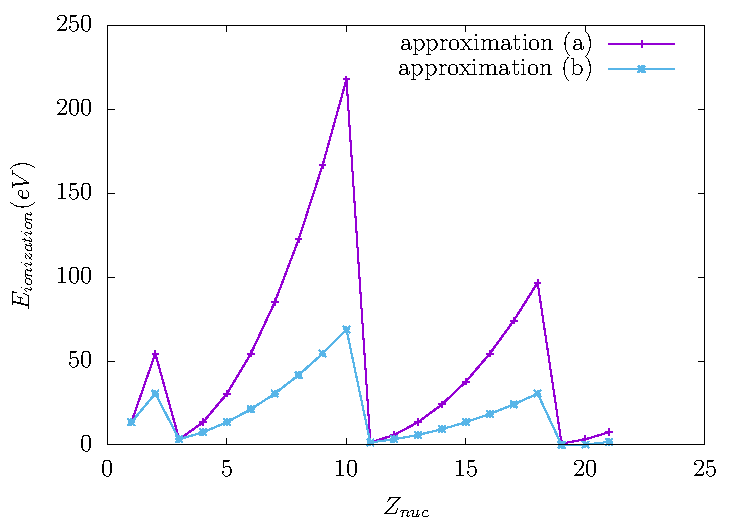
\includegraphics[width=.4\textwidth]{1-E-Z.pdf}
                \caption{1-21号元素的电离能}
                \label{1-E-Z}
            \end{figure}
            \\对于更高原子序数的情况,上述的简单近似失效,这是因为对于一些过渡金属来说,虽然从填充顺序的角度来说,他们的外层电子为$d$层电子,但是真正电离的时候,离开原子的确实主量子数小$1$的$s$层电子.
        \end{itemize}
    \end{enumerate}
\end{sol}

\begin{prob}[(5.3) \textbf{Exceptions to Madelung's Rule}]
    Although Madelung's rule for the filling of electronic shells holds extremely well, there are a number of exceptions to the rule. Here are a few of them:
    \begin{align*}
        \text{Cu}=&[\text{Ar}]4\text{s}^13\text{d}^{10}\\
        \text{Pd}=&[\text{Kr}]5\text{s}^04\text{d}^{10}\\
        \text{Ag}=&[\text{Kr}]5\text{s}^14\text{d}^{10}\\
        \text{Au}=&[\text{Xe}]6\text{s}^14\text{f}^{14}5\text{d}^{10}
    \end{align*}
    \item[$\triangleright$] What should the electron configuration be if these elements followed Madelung's rule and the Aufbau principle?
    \item[$\triangleright$] Explain how the statement "3d is inside of 4s" might help justify this exception in copper.
\end{prob}
\begin{sol}
    \begin{itemize}
        \item[$\triangleright$] 若电子排布遵从Madelung's rule和Aufbau principle,上面的元素的电子层结构应为
        \begin{align*}
            \text{Cu}=&[\text{Ar}]4\text{s}^23\text{d}^9\\
            \text{Pd}=&[\text{Kr}]5\text{s}^24\text{d}^8\\
            \text{Ag}=&[\text{Kr}]5\text{s}^24\text{d}^9\\
            \text{Au}=&[\text{Xe}]6\text{s}^24\text{f}^{14}5\text{d}^9
        \end{align*}
        \item[$\triangleright$] 由于3d比4s更靠近原子核,因此能量更低,根据Aufbau principle,应当先填充3d轨道.
    \end{itemize}
\end{sol}

\begin{prob}[(6.2) \textbf{Covalent Bonding in Detail$^*$}]
    \begin{enumerate}
        \item[(a)] \textit{Linear Combination of Atomic Orbitals}:\\\
        In Section 6.2.2 we considered two atoms each with a single atomic orbital. We called the orbital $\lvert 1\rangle$ around nucleus $1$ and $\lvert 2\rangle$ around nucleus $2$. More generally we may consider any set of wavefunctions $\lvert n\rangle$ for $n=1,\dots,N$. For simplicity, let us assume this basis is orthonormal $\langle n\vert m\rangle=\delta_{n,m}$ (More generally, one cannot assume that the basis set of orbitals is orthonormal. In Exercise 6.5 we properly consider a non-orthonormal basis.)\\
        Let us write a trail wavefunction for our ground state as
        \[
            \lvert\Psi\rangle=\sum_n\phi_n\lvert n\rangle.
        \]
        This is known as a linear combination of atomic orbitals, LCAO, or tight binding (it is used heavily in numerical simulation of molecules).\\
        We would like to find the lowest-energy wavefunction we can constract in this form, i.e., the best approximation to the actual ground-state wavefunction. (The more states we use in our basis, generally, the more accurate our result will be.) We claim that the ground state is given by the solution of the effective Schroedinger equation
        \[
            \mathcal{H}\phi=E\phi\tag{6.13}
        \]
        where $\phi$ is the vector of $N$ coefficients $\phi_n$, and $\mathcal{H}$ is the $N$ by $N$ matrix
        \[
            \mathcal{H}_{n,m}=\langle n\lvert\mathcal{H}\rvert m\rangle
        \]
        with $H$ the Hamiltonian of the full system we are considering. To prove this, let us construct the energy
        \[
            E=\frac{\langle\psi\lvert H\rvert\psi\rangle}{\langle\psi\vert\psi\rangle}
        \]
        \begin{itemize}
            \item[$\triangleright$] Show that minimizing this energy with respect to each $\phi_n$ gives the same eigenvalue equation, Eq. 6.13. (Caution: $\phi_n$ is the generally complex! If you are not comfortable with complex differentiation, write everything in terms of real and imaginary parts of each $\phi_n$.) Similarly, the second eigenvalue of the effective Schroedinger equation will be an approximation to first excited state of the system.
        \end{itemize}
        \item[(b)] \textit{Two-orbital covalent bond}\\
        Let us return to the case where there are only two orbitals in our basis. This pertains to a case where we have two identical nuclei and a single electron which will be shared between them to form a covalent bond. We wirte the full Hamiltonian as
        \[
            H=\frac{\bm{p}^2}{2m}+V(\bm{r}-\bm{R}_1)+V(\bm{r}-\bm{R}_2)=K+V_1+V_2
        \]
        where $V$ is the Coulomb interaction between the electron and the nucleus, $R_1$ is the position of the first nucleus and $R_2$ is the position of the second nucleus. Let $\epsilon$ be the energy of the atomic orbital around one nucleus in the absence of the other. In other words
        \begin{gather*}
            (K+V_1)\lvert 1\rangle=\epsilon\lvert 1\rangle\\
            (K+V_2)\lvert 2\rangle=\epsilon\lvert 2\rangle
        \end{gather*}
        Define also the cross-energy element
        \[
            V_{cross}=\langle 1\lvert V_2\rvert 1\rangle=\langle 2\lvert V_2\rvert 2\rangle
        \]
        and the hopping matrix element
        \[
            t=-\langle 1\lvert V_2\rvert 2\rangle=-\langle 1\lvert V_1\rvert 2\rangle
        \]
        These are not typos!
        \begin{itemize}
            \item[$\triangleright$] Why can we write $V_{cross}$ and $t$ equivalently using either one of the expressions given on the right-hand side?
            \item[$\triangleright$] Show that the eigenvalues of our Schroedinger equation Eq. 6.13 are given by
            \[
                E=\epsilon+V_{cross}\pm|t|
            \]
            \item[$\triangleright$] Argue (perhaps using Gauss's law) that $V_{cross}$ should roughly cancel the repulsion between nuclei, so that, in the lower eigenstate the total energy is indeed lower when the atoms are closer together.
            \item[$\triangleright$] This approximation must fail when the atoms get sufficiently close. Why?
        \end{itemize}
    \end{enumerate}
\end{prob}
\begin{sol}
    \begin{enumerate}
        \item[(a)] 
        \begin{itemize}
            \item[$\triangleright$] 系统能量为
            \begin{equation}
                E=\frac{\langle\psi\lvert H\rvert\psi\rangle}{\langle\psi\vert\psi\rangle}=\frac{\sum_{m,n}\phi_n^*\mathcal{H}_{nm}\phi_m}{\sum_n\abs{\phi_n}^2}.
            \end{equation}
            上式最小值为基态能量,其满足
            \begin{gather}
                0=\frac{\partial E}{\partial\phi_n^*}=\frac{\sum_m\mathcal{H}_{nm}}{\sum_p\abs{\phi_p}^2}-\left(\frac{\sum_{nm}\phi_n^*\mathcal{H}_{nm}\phi_m}{\sum_p\abs{\phi_p}^2}\right)\frac{\phi_n}{\sum_p\abs{\phi_p}^2}=\frac{\sum_m\mathcal{H}_{nm}}{\sum_p\abs{\phi_p}^2}-E\frac{\phi_n}{\sum_p\abs{\phi_p}^2},\quad\forall n,\\
                \Longrightarrow 0=\sum\mathcal{H}_{nm}-E\phi_n,\quad\forall n,\\
                \Longrightarrow \mathcal{H}\phi=E\phi.
            \end{gather}
            与式6.13相同.
        \end{itemize}
        \item[(b)] 
        \begin{itemize}
            \item[$\triangleright$] 因为两个原子是相同的,根据系统对称性,右边的两种形式均可以表示$V_{cross}$和$t$.
            \item[$\triangleright$] 系统哈密顿在$\{\lvert 1\rangle,\rvert 2\rangle\}$表象上可表为
            \begin{equation}
                \mathcal{H}=\left(\begin{matrix}
                    \epsilon+V_{cross}&-t\\
                    -t^*&\epsilon+V_{cross}
                \end{matrix}\right).
            \end{equation}
            该矩阵的本征值即为系统的本征能量,下面来求本征值. 该矩阵对应的特征方程为
            \begin{equation}
                \det(\mathcal{H}-EI)=\left\lvert\begin{matrix}
                    \epsilon+V_{cross}-E&-t\\
                    -t^*&\epsilon+V_{cross}-E
                \end{matrix}\right\rvert=(\epsilon+V_{cross}-E)^2-\abs{t}^2=0.
            \end{equation}
            解得系统的本征能量为
            \begin{equation}
                E=\epsilon+V_{cross}\pm\abs{t}.
            \end{equation}
            \item[$\triangleright$] $V_{cross}$的物理意义是电子处在1号原子的基态轨道上时与2号原子核间的库仑势,此时电子的概率幅是以1号原子核为球心成球对称分布,1号原子的基态轨道的有效半径小于两个原子核的间距,此时计算2号原子核处的电场,可以将1号原子核和电子视为一个整体(净电荷近似可认为零)考虑以1号原子核为半径,两原子核间距为半径的球面,根据高斯定理,这个球面上的电场以及这个球面以外的电场等于零,因此2号原子核的库仑势也就等于零,也就是说1号原子核对2号原子核的排斥与电子对2号原子核的吸引相抵消.
            \item[$\triangleright$] 当两个原子核靠得足够近,上面的近似就不成立了,因为如果1号原子基态上的电子有相当的概率跑到与1号原子距离大于两原子核间距的地方,那么还是根据高斯定理,计算2号原子核处的电场时球面内包裹的净电荷就偏正,2号原子核处以及稍远一些处的电场将都不为零,从而2号原子核的库仑势不为零,也就是说1号原子核对2号原子核的排斥会比电子对2号原子核的吸引要强.
        \end{itemize}
    \end{enumerate}
\end{sol}

\begin{prob}[(6.3) \textbf{LCAO and the Ionic-Covalent Crossover}]
    For exercise 6.2.b consider now the case where the atomic orbitals $\lvert 1\rangle$ and $\lvert 2\rangle$ have unequal energies $\epsilon_{0,1}$ and $\epsilon_{0,2}$. As the difference in these two energies increases show that the bonding orbital becomes more localized on the lower-energy atom. For simplicity you may use the orthogonality assumption $\langle 1\vert 2\rangle=0$. Explain how this calculation can be used to describe a crossover between covalent and ionic bonding.
\end{prob}
\begin{sol}
    根据题设,系统的哈密顿在$\{\lvert 1\rangle,\lvert 2\rangle\}$表象上的矩阵应表为
    \begin{equation}
        \mathcal{H}=\left(\begin{matrix}
            \epsilon_1&-t\\
            -t^*&\epsilon_2
        \end{matrix}\right),
    \end{equation}
    其中$\epsilon_1=\epsilon_{0,1}+V_{cross}$,$\epsilon_2=\epsilon_{0,2}+V_{cross}$. 该矩阵对应的特征方程为
    \begin{equation}
        \det(\mathcal{H}-EI)=\left\lvert\begin{matrix}
            \epsilon_1-E&-t\\
            -t^*&\epsilon_2-E
        \end{matrix}\right\rvert=(\epsilon_1-E)(\epsilon_2-E)-t^2=0.
    \end{equation}
    解得系统的本征能量为
    \begin{equation}
        E_{\pm}=\frac{1}{2}\left[(\epsilon_1+\epsilon_2)\pm\sqrt{(\epsilon_1-\epsilon_2)^2+4t^2}\right].
    \end{equation}
    将上述本征能量代入式
    \begin{equation}
        \mathcal{H}\psi=E\psi
    \end{equation}
    再归一化后可解得本征矢
    \begin{equation}
        \psi_{\pm}=\frac{1}{\sqrt{8t^2+2(\epsilon_2-\epsilon_1)^2\pm 2(\epsilon_2-\epsilon_1)\sqrt{(\epsilon_2-\epsilon_1)^2+4t^2}}}\left(\begin{matrix}
            -2t\\
            (\epsilon_2-\epsilon_1)\pm\sqrt{(\epsilon_2-\epsilon_1)^2+4t^2}
        \end{matrix}\right)
    \end{equation}
    其中"$-$"代表的是基态,"$+$"代表的是激发态. 不失一般性,假设$\epsilon_1<\epsilon_2$,当电子处于基态时,对其进行测量,有$\frac{4\abs{t}^2}{(\sqrt{\dots})^2}$的概率发现电子处于$\lvert 1\rangle$,有$\frac{2(\epsilon_2-\epsilon_1)^2+4t^2-2(\epsilon_2-\epsilon_1)\sqrt{(\epsilon_2-\epsilon_1)^2+4t^2}}{(\sqrt{\dots})^2}$,比较知$4t^2>2(\epsilon_2-\epsilon_1)^2+4t^2-2(\epsilon_2-\epsilon_1)\sqrt{(\epsilon_2-\epsilon_1)^2+4t^2}$,也就是说电子的轨道更集中在能量低的原子那一侧.\\
    这一计算结果可以解释共价键和离子键的差异:形成共价键的元素电负性相近,也就是说两个原子的基态能量差小,所以电子并没有很严重地偏向某个原子;而形成离子键的元素电负性相差较大,也就是说两个原子的基态能量差大,因此电子会很明显地集中在能量低(电负性强)的原子那一侧,这样一来,能量低的原子会带上负电,另一个原子会带上正电,从而通过库仑力形成离子键.
\end{sol}

\begin{prob}[(6.4) \textbf{Ionic Bond Energy Budget}]
    The ionization energy of a sodium atom is about $5.14$ eV. The electron affinity of a chlorine atom is about $3.62$ eV. When a single sodium atom bonds with a single chlorine atom, the bond length is roughly $0.236$ nm. Assuming that the cohesive energy is purely Coulomb energy, calculate the total energy released when a sodium atom and a chlorine atom come together to form a NaCl molecule. Compare your result to the experimental value of $4.26$ eV. Qualitatively account for the sign of your error.
\end{prob}
\begin{sol}
    钠离子和氯离子间的内聚能为
    \begin{equation}
        E_{coh}=\frac{e^2}{4\pi\epsilon_0d}=9.75\times 10^{-19}\text{J}=6.10e\text{V}.
    \end{equation}
    一个钠原子和一个氯原子形成氯化钠的过程释放能量
    \begin{equation}
        E=-5.14e\text{V}+3.63e\text{V}+6.10e\text{V}=4.59e\text{V}.
    \end{equation}
    这一计算结果比实验值稍大,这是因为在钠离子和氯离子相结合的时候还需要克服一些同性电荷之间的排斥力,这导致实际释放的能量应该比计算结果更小.
\end{sol}
\end{document}